%%%%%%%%%%%%%%%%%%%%%%%%%%%%%%%%%%%%%%%%%%%%%%%%%%%%%%%%%%%%%%%%%%%%%%
% Lớp 10 | Bất phương trình bậc 2 một ẩn | Giải bất phương trình bậc 2 một ẩn
% Dạng 0D7?2-6: Bài toán có tham số 𝑚
% Số câu: 23  (sinh tự động bởi tach_cau.py; từ nay thầy sửa trực tiếp file này)
%%%%%%%%%%%%%%%%%%%%%%%%%%%%%%%%%%%%%%%%%%%%%%%%%%%%%%%%%%%%%%%%%%%%%%

%%%%%%%%%%%%%%%% TRẮC NGHIỆM 4 PHƯƠNG ÁN %%%%%%%%%%%%%%%%

% nguồn: MaHoaNH_TracNghiem_Lop10
\begin{ex}%[0D7N2-6]%[ma:1391103d]
	Có bao nhiêu giá trị nguyên âm của tham số $m$ để  hàm số $y=\sqrt{x^2-2mx-2m+3}$ có tập xác định là $\mathbb{R}$.
	 \choice
		{$4$} 
		 {$6$}
		{\True  $3$}
		{$5$} 
	 \loigiai{
		Hàm số $y=\sqrt{x^2-2mx-2m+3}$ có  tập xác định là $\mathbb{R}$ khi $x^2-2mx-2m+3 \geq 0$ với mọi $x \in \mathbb{R}$\\
		$\Leftrightarrow \heva{ 
		&\Delta' \leq  0\\
		 &a>0}
		\Leftrightarrow  \heva{
		 &m^2+2m-3 \leq 0\\
		&1>0} 
		\Leftrightarrow -3 \leq m \leq  1$.\\
		Do  $m$ nguyên âm nên $m \in\{-3;-2;-1\}$.\\
		 Vậy có $3$ giá trị nguyên âm của $m$ thỏa yêu cầu bài toán.
	} 
\end{ex}

% nguồn: MaHoaNH_TracNghiem_Lop10
\begin{ex}%[0D7H2-6]%[ma:ab021d9c]
	Cho hàm số $f(x)=x^2-2x+m$. Với giá trị nào của tham số $m$ thì $f(x) \geq  0$, $\forall x \in \mathbb{R}$.
	 \choice
		{\True $m  \geq 1$}
		 {$m>1$}
		{$m>0$} 
		 {$m<2$}
	 \loigiai{
		Ta có $f(x) \geq 0$, $\forall x \in \mathbb{R}  \Leftrightarrow \heva{
		&a=1>0\\ 
		&\Delta'=1-m \leq  0}
		\Leftrightarrow  m \geq 1$.
	} 
\end{ex}

% nguồn: MaHoaNH_TracNghiem_Lop10
\begin{ex}%[0D7V2-6]%[ma:e2108153]
	 Phương trình $(m^2-4)x^2+2(m-2)x+3=0$ vô nghiệm khi và chỉ khi
	 \choice
		{\True $\hoac{&m\geq 2\\&m<-4}$} 
		 {$\hoac{&m>2\\&m<-4}$}
		{$-4<m\leq  2$}
		{$-4\leq m\leq  2$}
	\loigiai{ 
		Ta có $m^2-4=0\Leftrightarrow\hoac{&m=2\\&m=-2.}$ 
		\begin{itemize}
			\item Trường hợp $1$: Nếu $m=2$ phương  trình trở thành $3=0$ vô nghiệm, nhận $m=2$.
			\item Trường hợp $2$: Nếu $m=-2$ phương trình trở  thành $-8x+3=0\Leftrightarrow x=\dfrac{3}{8}$, loại $m=-2$.
			 \item Trường hợp $3$: Nếu $\heva{&m\neq 2\\&m\neq -2.}$\\
			 Ta có $\Delta'=(m-2)^2-3(m^2-4)=-2m^2-4m+16$.\\
			$\Delta'=0\Leftrightarrow\hoac{&m=2\\&m=-4.}$ 
			\begin{center}
				\begin{tikzpicture}[font=\footnotesize,line join=round,line cap=round,>=stealth]
						\tkzTabInit[nocadre=false,lgt=1.2,espcl=2.5,deltacl=0.5] 
						{$m$ /0.75,$\Delta'$/0.75} 
						{$ -\infty $,$ -4 $,$ 2  $,$ +\infty $}
						 \tkzTabLine{,-,0,+,0,-,}
					\end{tikzpicture}
			\end{center}
			Phương trình vô nghiệm $\Leftrightarrow \Delta'<0\Leftrightarrow  \hoac{&m<-4\\&m>2.}$
		\end{itemize}
		Vậy phương  trình vô nghiệm $\Leftrightarrow \hoac{&m\geq 2\\&m<-4.}$
	 }
\end{ex}


%%%%%%%%%%%%%%%% ĐÚNG/SAI %%%%%%%%%%%%%%%%

% nguồn: MaHoaNH_DungSai_Lop10
\begin{ex}%[0D7H2-6]%[ma:c91f0d2f]
	Cho bất phương trình bậc hai $-x^2+3x+1-m  \leq 0$, với $m$ là tham số thực.
	 \choiceTF
		 {\True Bất phương trình đã cho có một nghiệm là $x=1$ khi $m\geq 3$}
		{Bất phương trình  đã cho có một nghiệm là $x=0$ khi $m\leq 1$}
		{Bất phương  trình đã cho có một nghiệm là $x=-1$ khi $m\leq-3$}
		{\True Bất  phương trình đã cho có một nghiệm là $x=-2$ khi $m\geq -9$}
	 \loigiai{
		\begin{itemchoice}
			\itemch Ta có $x=1$ là một nghiệm của bất phương trình đã cho  nên $-1^2+3\cdot 1+1-m\leq 0$ hay $m\geq 3$.
			\itemch Ta có $x=0$ là một nghiệm của bất phương trình đã cho nên $-0^2+3\cdot  0+1-m\leq 0$ hay $m\geq 1$.
			\itemch  Ta có $x=-1$ là một nghiệm của bất phương trình đã cho nên $-(-1)^2+3\cdot (-1)+1-m\leq 0$ hay $m\geq -3$.
			\itemch Ta có $x=-2$  là một nghiệm của bất phương trình đã cho nên $-(-2)^2+3\cdot (-2)+1-m\leq 0$ hay $m\geq -9$.
		\end{itemchoice}
	 }
\end{ex}

% nguồn: MaHoaNH_DungSai_Lop10
\begin{ex}%[0D7H2-6]%[ma:bfb22f46]
	Cho hàm số $f(x)=x^2+2mx+3m-2$ ($m$ là  tham số). Xét tính đúng sai của các mệnh đề sau.
	\choiceTF 
		{\True Khi $m=4$ thì bất phương trình  $f(x)\geq 0$ có tập nghiệm là $\left(-\infty;-4-\sqrt{6}\right]\cup\left[-4+\sqrt{6};+\infty\right)$}
		{$f(x)\geq 0,\forall  x\in\mathbb{R}$ khi $m\in(-\infty;1)\cup(2;+\infty)$}
		{\True $x=1$ là một nghiệm  của bất phương trình $f(x)\geq 0$ khi $m\in\left[\dfrac{1}{5};+\infty\right)$}
		{Với $m=2$ thì đồ thị hàm số  $f(x)$ cắt trục hoành tại hai điểm phân biệt}
	\loigiai{ 
		\begin{itemchoice}
			\itemch Đúng. Vì $m=4$, ta có bất phương trình  $x^2+8x+10\geq 0\Leftrightarrow m\in\left(-\infty;-4-\sqrt{6}\right]\cup\left[-4+\sqrt{6};+\infty\right)$.
			\itemch Sai. Vì $x^2+2mx+3m-2\geq 0,\forall x\Leftrightarrow m^2-3m+2\leq 0\Leftrightarrow  m\in[1;2]$.
			\itemch Đúng. Vì $x=1$, ta có $1^2+2m\cdot 1+3m-2\geq 0\Leftrightarrow 5m-1\geq  0\Leftrightarrow m\in\left[\dfrac{1}{5};+\infty\right)$.
			\itemch Sai. Vì $m=2$, ta có $f(x)=x^2+4x+4=0$ có nghiệm kép. Khi đó đồ thị hàm số tiếp xúc với trục hoành tại điểm  $x=-2$.
		\end{itemchoice}
	 }
\end{ex}

% nguồn: MaHoaNH_DungSai_Lop10
\begin{ex}%[0D7H2-6]%[ma:5f1500a3]
	Cho bất  phương trình bậc hai $2x^2+x+m-2>0$, với $m$ là tham số thực.
	 \choiceTF
		{Bất phương trình  đã cho có một nghiệm là $x=1$ khi $m>1$}
		{\True Bất phương trình đã cho  có một nghiệm là $x=0$ khi $m>2$}
		{\True Bất phương trình đã cho có một  nghiệm là $x=-1$ khi $m>1$}
		{Bất phương trình đã cho có một nghiệm là $x=2$ khi  $m<-8$}
	 \loigiai{
		\begin{itemchoice}
			\itemch Ta có  $x=1$ là một nghiệm của bất phương trình đã cho nên $2\cdot 1^2+1+m-2>0$ hay $m>-1$.
			\itemch Ta có $x=0$  là một nghiệm của bất phương trình đã cho nên $2\cdot 0^2+0+m-2>0$ hay $m>2$.
			\itemch Ta có $x=-1$ là một nghiệm của bất phương trình đã cho nên $2\cdot(-1)^2-1+m-2>0$  hay $m>1$.
			\itemch Ta có $x=2$  là một nghiệm của bất phương trình đã cho nên $2\cdot 2^2+2+m-2>0$ hay $m>-8$.
		\end{itemchoice}
	 }
\end{ex}

% nguồn: MaHoaNH_DungSai_Lop10
\begin{ex}%[0D7V2-6]%[ma:163207e1]
	Cho $f(x)=x^2-2(m+1)x+4$ với $m$ là tham số thực. 
	\choiceTF 
		{\True $f(x)$ là tam thức bậc hai với mọi  giá trị của tham số $m$}
		{\True Khi $m=1$ thì hàm số $y=\sqrt{f(x)}$ có tập xác  định là $\mathbb{R}$}
		{Khi $m=-\dfrac{1}{2}$ thì  $f(x)<0,\forall x\in[-2;3]$}
		{Có $2$ giá trị nguyên  âm của tham số $m$ để $f(x)>0,\forall x\in\mathbb{R}$}
	 \loigiai{
		\begin{itemchoice}
			\itemch \textbf{Đúng}. 
			 \itemch \textbf{Đúng}. \\
			Với $m=1$ thì $y=\sqrt{f(x)}=\sqrt{x^2-4x+4}$ có ĐKXĐ  $x^2-4x+4\ge 0 \Leftrightarrow x\in \mathbb{R}$.
			\itemch  \textbf{Sai}. \\
			Với  $m=-\dfrac{1}{2}$ thì $f(x)=x^2-x+4<0 \Leftrightarrow x\in \varnothing$.
			 \itemch \textbf{Sai}. \\
			$f(x)>0,\forall x\in\mathbb{R} \Leftrightarrow \heva{&a>0  \\ &\Delta<0} \Leftrightarrow 4(m+1)^2-16<0 \Leftrightarrow -3<m<1$. \\
			Vậy có $3$ giá trị  nguyên $m\in\{-2;-1;0\}$.
		\end{itemchoice}
	 }
\end{ex}


%%%%%%%%%%%%%%%% TRẢ LỜI NGẮN %%%%%%%%%%%%%%%%

% nguồn: MaHoaNH_TraLoiNgan_Lop10
\begin{bt}%[0D7H2-6]%[ma:bc748875]
	Năm $2003$, nhiệt độ ngày tại Death Valley (Thung Lũng Chết) của bang California được xác định qua hàm số $t(d)=-0{,}0018d^2+0{,}657d+50{,}95$, trong đó $t$ là nhiệt độ tính theo độ Fahrenheit $(^\circ F)$ và  $d$ là ngày trong năm tính từ $1/1/2003$. Nhiệt độ cao nhất trong năm đó là bao nhiêu độ $F$ (tính đến hàng đơn vị)?
	 \shortans{111}
	 \loigiai{
		Vì $t(d)=-0{,}0018d^2+0{,}657d+50{,}95$ là hàm số bậc hai có  hệ số $a=-0{,}0018<0$ nên $t(d)$ đạt giá trị lớn nhất tại $d=-\dfrac{b}{2a}=-\dfrac{0{,}657}{2\cdot (-0{,}0018)}=182{,}5 $.\\
		Giá trị lớn  nhất là $t\approx 111^\circ F$.\\
		Vậy nhiệt độ cao nhất là $111^\circ F$ vào  ngày thứ $182$.
	 }
\end{bt}

% nguồn: MaHoaNH_TraLoiNgan_Lop10
\begin{bt}%[0D7H2-6]%[ma:02f9ab20]
	Có bao nhiêu giá trị nguyên của $m\in [0;30]$ để bất phương trình $x^2-(m+2)x+8m+1\le 0$ vô nghiệm? 
	\shortans{2} 
	\loigiai{ 
		Bất phương trình $x^2-(m+2)x+8m+1\le 0$  vô nghiệm khi và chỉ khi $x^2-(m+2)x+8m+1>0$, $\forall x\in \mathbb{R}$.\\
		Điều kiện $\Delta<0\Leftrightarrow (m+2)^2-4(8m+1)>0\Leftrightarrow m^2-28m>0\Leftrightarrow \hoac{&m<0\\&m>28.}$\\ 
		Kết hợp điều kiện $m\in[0;30]$  và $m$ là số nguyên suy ra $m\in \{29;30\}$.\\
		 Vậy có $2$ giá trị thỏa mãn.
	} 
\end{bt}

% nguồn: MaHoaNH_TraLoiNgan_Lop10
\begin{bt}%[0D7H2-6]%[ma:8b30459e]
	Có bao nhiêu  giá trị nguyên của tham số $m$ thuộc đoạn $\left[-10;5\right]$ để phương trình $x^2-(m+1)x+3m-5=0$ có hai nghiệm phân biệt?
	 \shortans{13}
	 \loigiai{
		Ta  có $\Delta=[-(m+1)]^2-4\cdot 1\cdot (3m-5)=m^2-10m+21$.\\
		Để phương trình $x^2-(m+1)x+3m-5=0$ có hai nghiệm phân  biệt thì \[\Delta > 0\text{ hay } m^2-10m+21> 0.\]
		Tam thức bậc hai $m^2-10m+21$ có  $a=1> 0$ và có hai nghiệm $m_1=3,m_2=7$.\\
		Do đó, $m^2-10m+21> 0$ khi $m\in (-\infty;3)\cup (7;+\infty)$.\\ 
		Mà $m\in  \mathbb{Z}$ và $m\in \left[-10;5\right]$ nên có $13$ giá trị nguyên của tham số $m$ thỏa mãn.
	} 
\end{bt}

% nguồn: MaHoaNH_TraLoiNgan_Lop10
\begin{bt}%[0D7H2-6]%[ma:9111cc2d]
	Có bao nhiêu giá trị  nguyên của $m$ để $f(x)=x^2-2(2 m-3) x+4 m-3>0$, với $\forall x \in \mathbb{R}$?
	 \\\shortans{1}
	\loigiai{ 
		Ta  có
		\allowdisplaybreaks 
		\begin{eqnarray*}
			f(x)=x^2-2(2 m-3) x+4 m-3>0, \forall x  \in \mathbb{R}&\Leftrightarrow&\heva{&a>0 \\& \Delta'<0} \\&\Leftrightarrow&\heva{&1>0 \\& (2 m-3)^2-(4 m-3)<0} \\&\Leftrightarrow& 4 m^2-16 m+12<0 \Leftrightarrow 1<m<3.
		\end{eqnarray*}
		Vậy chỉ có một giá trị nguyên $m=2$ thỏa mãn yêu  cầu bài toán.
	 }
\end{bt}

% nguồn: MaHoaNH_TraLoiNgan_Lop10
\begin{bt}%[0D7H2-6]%[ma:f8e695a7]
	Có bao nhiêu giá trị nguyên của tham số $m$ để hàm số $y=\sqrt{x^2+2mx+4m+5}$ xác  định với mọi $x\in\mathbb{R}$?
	\shortans{7} 
	 \loigiai{
		 Hàm số $y=\sqrt{x^2+2mx+4m+5}$ xác định với mọi $x\in\mathbb{R}$ khi và chỉ khi
		\begin{eqnarray*}
			&&x^2+2mx+4m+5\geq 0,\forall x\in\mathbb{R}\\ 
			 &\Leftrightarrow&\heva{&a=1>0\\&\Delta'=m^2-4m-5\leq 0}\\
			 &\Leftrightarrow& -5\leq m\leq 1.
		\end{eqnarray*}
		Vậy có $7$ giá trị nguyên của tham số $m$  thỏa mãn.
	} 
\end{bt}

% nguồn: MaHoaNH_TraLoiNgan_Lop10
\begin{bt}%[0D7V2-6]%[ma:4319d30d]
	Tìm  số nguyên âm $m$ lớn nhất sao cho $-x^2+2(m+1)x-m^2+m < 0$ với mọi $x\in \mathbb{R}$.
	\shortans{-1} 
	\loigiai{ 
		Xét tam thức bậc hai $f(x)=-x^2+2(m+1)x-m^2+m$  có \[\Delta '=\left(m+1\right)^2-\left(-1\right).\left(-m^2+m\right)=3m+1\text{ và }a=-1< 0.\]
		Để $f(x) < 0$ với mọi $x\in \mathbb{R}$ thì $\Delta '=3m+1< 0$  suy ra $m < \dfrac{-1}{3}$.
	} 
\end{bt}

% nguồn: MaHoaNH_TraLoiNgan_Lop10
\begin{bt}%[0D7V2-6]%[ma:3080a6c3]
	Có bao nhiêu giá  trị nguyên của $m \in[0; 30]$ để bất phương trình $x^2-(m+2) x+8m+1\leq 0$ vô nghiệm?
	\shortans{2} 
	\loigiai{ 
		Bất phương trình $x^2-(m+2) x+8m+1\leq  0$ vô nghiệm
		khi và chỉ khi $x^2-(m+2) x+8m+1>  0$, $\forall x \in \mathbb{R}$. Điều này tương đương với
		$$\Delta < 0\Leftrightarrow(m+2)^2-4(8m+1) > 0\Leftrightarrow m^2-28m > 0\Leftrightarrow\hoac{&m < 0\\&m >  28.}$$
		Kết hợp điều kiện $m \in[0; 30]$ và $m\in\mathbb{Z}$, ta được $m\in\{29; 30\}$  nên có $2$ giá trị thỏa mãn.
	} 
\end{bt}

% nguồn: MaHoaNH_TraLoiNgan_Lop10
\begin{bt}%[0D7V2-6]%[ma:c590a38a]
	Có bao nhiêu giá trị nguyên của  tham số $m$ thuộc đoạn $\left[-20;30\right]$ để bất phương trình $x^2+2mx+m-2< 0$ nghiệm đúng với mọi $x\in (1;2)$?
	 \shortans{20}
	\loigiai{ 
		Tam thức bậc hai $f(x)=x^2+2mx+m-2$ có  \[\Delta'=m^2-m+2=\left(m-\dfrac{1}{2} \right)^2+\dfrac{7}{4} \ge \dfrac{7}{4} > 0,\,\forall m\in \mathbb{R}.\]
		Do đó $f(x)$ có hai nghiệm phân biệt $x_1, x_2\,\left(x_1 < x_2 \right)$ với mọi $m\in  \mathbb{R}$.\\
		Để $f(x) < 0$ với mọi $x\in (1;2)$ thì $x_1 \le 1< 2\le x_2$ \[\Leftrightarrow  \heva{&f(1)\leq 0\\&f(2)\leq 0}\Leftrightarrow\heva{&3m-2\leq 0\\&5m+2\leq 0}\Rightarrow m\leq -\dfrac{2}{5}.\]
		Vậy có $20$ giá trị nguyên của tham số $m$ thuộc đoạn $\left[-20;30\right]$ thỏa  mãn yêu cầu bài toán.
	} 
\end{bt}

% nguồn: MaHoaNH_TraLoiNgan_Lop10
\begin{bt}%[0D7V2-6]%[ma:4af3cf77]
	Tìm tất  cả các giá trị nguyên của tham số $m$ thuộc đoạn $\left[-9;10\right]$ để \break$f(x)=x^2+2(m-1)x+m^2-m+1$ không âm với mọi $x\in \mathbb{R}$.
	 \shortans{11}
	 \loigiai{
		Ta  có $a=1,b=2(m-1),c=m^2-m+1,b^{{'}}=\dfrac{b}{2}=m-1$.\\
		Theo giả thiết $f(x)\ge 0,\forall  x\in \mathbb{R}\Leftrightarrow \heva{&{a > 0} \\
		&{\Delta'\le 0}}\Leftrightarrow \heva{&{a=1> 0\text{ (luôn đúng)}} \\ 
		&{(m-1)^2-\left(m^2-m+1\right)\le  0}
		&}$\\ $\Leftrightarrow m^2-2m+1-m^2+m-1\le 0\Leftrightarrow m\ge  0$.\\
		Mà $m\in\left[-9;10\right]$ nên  $m\in\{0;1;\ldots;10\}$.\\
		Vậy có $11$ giá trị nguyên của tham  số $m$ thỏa mãn yêu cầu bài toán.
	} 
\end{bt}

% nguồn: MaHoaNH_TraLoiNgan_Lop10
\begin{bt}%[0D7V2-6]%[ma:14f56191]
	Có bao nhiêu giá trị nguyên của  tham số $m$ trong đoạn $[-10;10]$ làm cho bất phương trình $(m-1)x^2+(m-1)x+m>0$ đúng với mọi $x$ thuộc $\mathbb{R}$.
	 \shortans{10}
	 \loigiai{
		\begin{itemize}
			\item[TH1:] $m=1$ khi  đó bất phương trình trở thành $1>0,\forall x\in\mathbb{R}$ nên $m=1$ thỏa mãn.
			\item[TH2:] $m\neq1$, bất phương trình $(m-1) x^2+(m-1) x+m>0$ đúng với  mọi $x$ thuộc $\mathbb{R}$
			\begin{eqnarray*}
				 &\Leftrightarrow&\heva{&m-1>0\\&\Delta<0}\Leftrightarrow\heva{&m>1\\&(m-1)^2-4(m-1)m<0}\\
				&\Leftrightarrow&\heva{&m>1\\&-3m^2+2m+1<0}\Leftrightarrow\heva{&m>1\\&{\hoac{&m<-\dfrac{1}{3}\\&m>1}}}\Leftrightarrow m>1. 
			\end{eqnarray*}
		\end{itemize}
		Kết hợp TH1 và TH2, vậy giá trị $m$ cần tìm là $m\geq 1$. Suy ra có $10$ giá trị nguyên của  $m$ thỏa mãn.
	 }
\end{bt}

% nguồn: MaHoaNH_TraLoiNgan_Lop10
\begin{bt}%[0D7V2-6]%[ma:07eeea80]
	Có bao nhiêu giá trị nguyên dương của tham số $m$ để  $f(x)=(m-1)x^2+2(m-1)x+m-3$ không dương với mọi $x\in \mathbb{R}$.
	\shortans{1} 
	\loigiai{ 
		Ta có $a=m-1$, $b=2(m-1)$, $b'=m-1$, $c=m-3$.\\ 
		Theo  giả thiết $(m-1)x^2+2(m-1)x+m-3\le 0,\forall x\in \mathbb{R}$.\tagEX{*}
		\begin{enumerate}[\bf TH1.]
			\item  $a=m-1=0\Rightarrow m=1$.\\
			Thay vào (*) ta được  $1-3\le 0,\forall x\in \mathbb{R}$ (đúng).
			Suy ra $m=1$ thỏa  mãn.
			\item  $a=m-1\ne 0\Rightarrow m\ne 1$.
			\begin{eqnarray*}
				 (*)&\Leftrightarrow& \heva{&a < 0 \\
				&\Delta' \le 0}\Leftrightarrow \heva{&m-1<  0 \\
				 &(m-1)^2-(m-1)(m-3)\le 0}\\
				&\Leftrightarrow& \heva{&m  < 1 \\
				&m^2-2m+1-(m^2-4m+3)\le 0}\Leftrightarrow \heva{&m  < 1 \\
				&2m-2\le  0}\Leftrightarrow \heva{&m < 1 \\
				 &m\le 1}\Leftrightarrow m < 1.
			\end{eqnarray*}
		\end{enumerate}
		Hợp hai kết quả trên, ta được $m\le 1$ thỏa  mãn đề bài.\\
		Vậy có $1$  giá trị nguyên dương của $m$ thỏa mãn yêu cầu bài toán.
	} 
\end{bt}


%%%%%%%%%%%%%%%% TỰ LUẬN %%%%%%%%%%%%%%%%

% nguồn: MaHoaNH_TuLuan_Lop10
\begin{bt}%[0D7H2-6]%[ma:46b00825]
	Có bao  nhiêu giá trị nguyên của tham số $m$ thuộc đoạn $\left[-5;8\right]$ để phương trình
	$$x^2 -  4mx + 4m^2 = 0$$
	có nghiệm  kép?
	 \loigiai{
		Phương trình: $x^2 - 4mx + 4m^2 =  0$\\
		Có $\Delta = (-4m)^2 - 4 \cdot 1 \cdot  4m^2 = 16m^2 - 16m^2 = 0$\\
		Luôn có nghiệm kép với mọi  $m$.\\
		Mà $m \in \mathbb{Z}  \cap [-5;8]$ có $14$ giá trị nguyên.\\
	 Vậy có $14$ giá trị nguyên của $m$ để phương trình có nghiệm kép.}
\end{bt}

% nguồn: MaHoaNH_TuLuan_Lop10
\begin{bt}%[0D7V2-6]%[ma:219f3f33]
	Có bao nhiêu giá trị nguyên của tham số $m$, hàm  số $y=\sqrt{x^2-2mx+m-1}$ có tập xác định là $\mathbb{R}$?
	\loigiai{ 
		Để hàm số $y=\sqrt{x^2-2mx+m-1}$  có tập xác định là $\mathbb{R}$ thì \[x^2-2mx+m-1\ge 0,\,\forall x\in \mathbb{R}\Leftrightarrow\heva{&{a > 0} \\
		&{\Delta  \le 0}&}\Leftrightarrow\heva{&1>0\\&m^2-m+1\leq 0\;(*)}.\]
		 Vì $\left(m-\dfrac{1}{2}\right)^2+\dfrac{3}{4}>0,\,\forall x$ nên (*) vô nghiệm.\\
		Vậy không tồn tại giá trị của tham số $m$ để thoả mãn yêu cầu bài  toán.
	 }
\end{bt}

% nguồn: MaHoaNH_TuLuan_Lop10
\begin{bt}%[0D7V2-6]%[ma:4272f6be]
	Có bao nhiêu giá trị nguyên của tham số $m$ thuộc  khoảng $\left(-50;50\right)$ để phương trình $x^2+(m-2)x-8m+1=0$ có hai nghiệm phân biệt?
	 \loigiai{
		Ta có  $a=1\ne 0,b=m-2,c=-8m+1$.\\
		Phương trình có hai nghiệm phân biệt khi và chỉ khi \[\Delta=(m-2)^2-4(-8m+1) > 0\Leftrightarrow m^2+28m > 0.\] 
		Xét  $m^2+28m=0\Leftrightarrow m=0$ hoặc $m=-28$.\\
		Bảng xét dấu 
		\begin{center}
			\begin{tikzpicture}[>=stealth]
					 \tkzTabInit[nocadre=false,lgt=1.5,espcl=2,deltacl=0.6]{$x$/.7,$f (x)$/.7}
						{$-\infty$,$0$,$28$,$+\infty$} 
					 \tkzTabLine{,+,$0$,-,$0$,+,}
				\end{tikzpicture}
		\end{center}
		Ta có $m^2+28m > 0\Leftrightarrow m\in (-\infty;-28)\cup (0;+\infty)$.\\ 
		Mà $m$ nguyên  thuộc khoảng $\left(-50;50\right)$ nên $m\in\{-49;-48;\ldots;-29\}\cup\{1;2;3;\ldots;49\}$.
		Vậy có $70$ giá trị nguyên của tham  số $m$ thỏa mãn yêu cầu bài toán.
	} 
\end{bt}

% nguồn: MaHoaNH_TuLuan_Lop10
\begin{bt}%[0D7V2-6]%[ma:fc4623ab]
	Có bao nhiêu giá trị nguyên dương của tham số $m$  để
	$$f(x) = x^2 + 2(m - 1)x + m  - 3$$
	luôn dương với mọi $x \in \mathbb{R}$? 
	\loigiai{ 
		Hàm số $f(x)$ là một tam thức bậc hai có hệ số  $a = 1 > 0$.\\
		 Để $f(x) > 0,\ \forall x \in \mathbb{R}$ thì cần và đủ:
		 \[
		\Delta  < 0.
		 \]
		Tính  biệt thức:
		\begin{align*}
			\Delta &= [2(m - 1)]^2  - 4 \cdot 1 \cdot (m - 3) \\
			&= 4(m - 1)^2 -  4(m - 3) \\
			&= 4\left[(m - 1)^2 - (m - 3)\right] \\ 
			&=  4\left[m^2 - 2m + 1 - m + 3\right] = 4(m^2 - 3m + 4)
		\end{align*}
		Xét điều kiện: 
		 \[
		\Delta < 0 \Leftrightarrow 4(m^2  - 3m + 4) < 0 \Leftrightarrow m^2 - 3m + 4 < 0
		 \]
		Xét tam thức $m^2 - 3m  + 4$, ta có:
		 \[
		\Delta' = (-3)^2 - 4 \cdot 1 \cdot 4 = 9 -  16 = -7 < 0
		\] 
		 Tam thức luôn dương với mọi $m \in \mathbb{R}$.\\
		Vậy $m^2 -  3m + 4 > 0,\ \forall m$ không tồn tại $m$ để $f(x)$ luôn dương.\\
		\textbf{Vậy có } $0$ \textbf{giá trị nguyên dương của $m$  thỏa mãn yêu cầu.}
	} 
\end{bt}

% nguồn: MaHoaNH_TuLuan_Lop10
\begin{bt}%[0D7C2-6]%[ma:617792e7]
	Tìm giá trị nguyên dương nhỏ nhất của tham số $m$ để bất phương trình \break$x^2+6x+m+7\le 0$ vô nghiệm. 
	 \loigiai{
		Ta có $x^2+6x+m+7\le 0$ vô nghiệm \[\Leftrightarrow x^2+6x+m+7> 0,\forall x\in \mathbb{R}\Leftrightarrow \heva{&{a > 0} \\&{\Delta'< 0}&}\Leftrightarrow \heva{&1>  0\text{ (luôn đúng)}\\&{3^2-(m+7) < 0}}\Leftrightarrow m > 2.\]
		Vậy với $m > 2$ thì bất phương trình $x^2+6x+m+7\le 0$ vô nghiệm. 
	} 
\end{bt}
